\documentclass[11pt,a4paper]{article}
\usepackage[utf8]{inputenc}
\usepackage[T1]{fontenc}
\usepackage{lmodern}
\usepackage[a4paper,margin=2.4cm]{geometry}
\usepackage{setspace,microtype,graphicx,booktabs,tabularx,array,longtable,enumitem,hyperref,xcolor,float,caption}
\usepackage{tikz}
\usepackage[backend=biber,style=authoryear,sorting=nyt,maxcitenames=2,maxbibnames=99]{biblatex}
\addbibresource{references.bib}
\usetikzlibrary{arrows.meta,positioning,shapes.geometric,calc}
\hypersetup{colorlinks=true,linkcolor=blue!50!black,citecolor=blue!50!black,urlcolor=blue!60!black,pdftitle={Responsible AI Technical Report: BrainWaveNet},pdfauthor={Levi Pedro Tejedor Rico}}
\setstretch{1.12}
\setlist[itemize]{leftmargin=*,itemsep=2pt,topsep=2pt}
\setlist[enumerate]{leftmargin=*,itemsep=2pt,topsep=2pt}
\newcolumntype{Y}{>{\raggedright\arraybackslash}X}
\newcommand{\ASD}{\textsc{asd}}
\newcommand{\TD}{\textsc{td}}
\newcommand{\PBG}{\textsc{pbg}}
\newcommand{\SUM}{\textsc{sum}}
\newcommand{\FAST}{\textsc{fast}}

\title{\textbf{Technical Report: Responsible AI Assessment of BrainWaveNet}\\
\large Responsible AI Assessment for Autism Spectrum Disorder Research}
\author{Levi Pedro Tejedor Rico\\Student ID: 4506001}
\date{Module: CSI\_7\_DEL -- Deep Learning}

\begin{document}
\maketitle

\begin{abstract}
This report assesses BrainWaveNet, a wavelet-based Transformer that classifies autism spectrum disorder (ASD) and typically developing participants using resting-state functional MRI. It combines Leslie's SUM values (Respect, Connect, Protect and Care), FAST principles (Fairness, Accountability, Sustainability and Transparency), and process-based governance across the AI lifecycle. BrainWaveNet is a research prototype evaluated on ABIDE-I; its reported performance and lack of external clinical validation do not support diagnostic use. The assessment identifies evidence gaps in stakeholder participation, subgroup evaluation, test-set governance, reproducibility and operational oversight. It proposes proportionate governance gates, accountable roles and social impact assessment checkpoints. The recommendation is to restrict the model to research until independent validation, meaningful autistic community participation and appropriate clinical safety governance have been demonstrated. It also identifies evidence requirements for reproducibility, human oversight and post-release review if clinical evaluation is proposed. Documented facts are distinguished from recommendations, and remaining limitations are recorded for future work.
\end{abstract}

\tableofcontents
\newpage

\section{Introduction}
This report evaluates whether BrainWaveNet is suitable for use in a human healthcare environment and examines what would be required for its responsible redevelopment. The project is a deep-learning research model that analyses resting-state functional magnetic resonance imaging (rs-fMRI) data to classify participants into an ASD group or a typically developing control group. The ethical question goes beyond technical classification: we must consider whether the model's purpose, evidence base, design choices and governance justify any real-world use that could affect autistic people.

To answer this, our evaluation applies Leslie's SUM values alongside the FAST principles, translating them directly into a process-based governance (PBG) framework spanning problem formulation, data acquisition, preprocessing, modelling, validation, and deployment. The report distinguishes between information explicitly documented in the published research and issues for which evidence is not available. The absence of information in a paper is treated as an evidence gap, not as proof of deliberate omission. Recommendations are therefore based on the evidence that is currently available.

The scope encompasses this specific model, dataset, and public code implementation, paying close attention to social impact, fairness, accountability, transparency, sustainability, privacy, clinical safety, and technical validity. Our analysis relies strictly on the BrainWaveNet paper, ABIDE-I documentation, and the linked public repository; we do not independently re-run experiments or handle identifiable participant data.

Naturally, this document is neither a clinical trial report, a formal legal opinion, nor a certified medical-device conformity assessment. We avoid inferring individual diagnostic capacity from group-level statistics, nor do we assume that the permissions governing a public research dataset automatically extend to new clinical applications. Where sources omit governance workflows, we log an evidence gap and propose safeguards rather than assuming misconduct. Section 2 outlines the clinical and technical context, Section 3 maps out the SUM/FAST assessment alongside lifecycle controls and decision gates, and Section 4 concludes with concrete recommendations for deployment.

\section{AI Project Background}
\subsection{Clinical and data context}
Autism is a heterogeneous neurodevelopmental condition. In clinical practice, identification involves developmental history and behavioural assessment. A neuroimaging classifier should not be treated as a standalone diagnostic tool or as a complete representation of an individual's support needs. Although neuroimaging research has identified group-level patterns of functional connectivity, substantial differences between individuals remain. This limits the extent to which group-level findings can be applied to individual diagnosis (\cite{holiga2019}).

The Autism Brain Imaging Data Exchange (ABIDE-I) aggregates structural and resting-state MRI scans alongside phenotypic metadata. Its baseline release encompassed 1,112 participants spanning 17 independent international sites, featuring 539 individuals with ASD and 573 typically developing controls aged roughly 7 to 64 years (\cite{dimartino2014,abidewebsite}). Multi-site datasets provide opportunities to study larger and more diverse groups, but they also introduce variation caused by differences in scanners, acquisition protocols, recruitment methods and participant characteristics. If these site-related differences are not properly addressed, they may affect neuroimaging results (\cite{abraham2017,abideharmonization2022}).

\subsection{BrainWaveNet method and reported evidence}
Jeong et al. (2024) introduce BrainWaveNet to extract spatiotemporal representations from rs-fMRI time series directly within the frequency domain. Their pipeline applies a complex Morlet continuous wavelet transform (CWT) to blood-oxygen-level-dependent signals. Residual convolutional blocks, frequency token encoders, and temporal Transformer layers subsequently process the resulting real and imaginary coefficients, while spatial attention and cross-attention mechanisms model complex relationships across regions of interest (ROIs). The final output is a binary classification between participants in the ASD group and participants in the typically developing control group. This describes the research task and should not be interpreted as evidence that the model can diagnose individuals (\cite{jeong2024}).

The authors utilize CPAC-preprocessed data featuring a 0.01--0.1 Hz band-pass filter, omitting global signal regression, while employing the Craddock 200 atlas with 78 time points per subject. The CWT representation splits data into five distinct frequency sub-bands, adjusting sampling frequencies dynamically to match site-specific repetition times. After the reported quality-control and exclusion procedures, the study includes 897 participants: 414 in the ASD group and 483 controls. The paper describes a 7:2:1 training, validation and test split, as well as five-fold cross-validation and model selection based on validation AUC. These procedures should be interpreted according to the exact experimental protocol reported by the authors (\cite{jeong2024}).

BrainWaveNet reports an AUC of 0.7388, an accuracy of 67.55\%, sensitivity of 66.49\% and specificity of 68.35\%. Although the model performs better than some baseline methods on AUC, accuracy and sensitivity, its specificity is lower than its sensitivity. The reported standard deviations for sensitivity and specificity are also considerable (9.17 and 9.80 percentage points, respectively). These results are retrospective research metrics. They do not demonstrate clinical utility, reliable individual risk estimates or improvements in patient care. The study does not report prospective clinical evaluation or independent external validation on a separate cohort (\cite{jeong2024}).

The public code repository allows the implementation to be inspected, but public availability does not guarantee that the experiments can be reproduced. Some repository outputs appear to differ from results reported in the paper. These differences require further investigation in a controlled environment before the results can be considered independently reproducible (\cite{brainwavenetcode}). The paper's ROI analysis should also be treated as exploratory. Attention weights do not, by themselves, establish biological causation or show that an intervention based on the model would benefit an individual. Technical pattern recognition must therefore be distinguished from clinical utility and improvements in care (\cite{topol2019,who2021}). Furthermore, reducing the diversity of autistic people to two classification groups does not capture the full range of their experiences, characteristics or support needs.

The system boundary therefore extends beyond the neural network itself. It includes the MRI scanner, local acquisition protocols, site-specific preprocessing, participant selection, the model's decision threshold, the professional interpreting the output and the institutional framework governing its use. Errors and biases may arise at any stage of this process, rather than only within the model architecture (\cite{suresh2021}). This system-level perspective informs the ethical assessment below.

\section{Responsible AI Assessment}
SUM considers affected people; FAST assesses operational properties. Lifecycle controls assign gaps to owners and decision points.

\subsection{SUM values}
Table~\ref{tab:sum} assesses Leslie's SUM values.

\begin{table}[H]
\centering
\caption{Assessment of BrainWaveNet against SUM values.}
\label{tab:sum}
\small
\begin{tabularx}{\textwidth}{p{2.1cm}Y Y}
\toprule
\textbf{Value} & \textbf{Evidence and assessment} & \textbf{Required response}\\
\midrule
Respect & The paper reports 414 autistic participants but no autistic co-design or influence over research aims and interpretation. Representation is not participation. Neuroimaging linked to phenotype remains sensitive. & Establish accessible, paid autistic participation in decisions; respect neurodiversity in language; follow data permissions, minimise access and prohibit re-identification.\\
Connect & ABIDE-I connects 17 sites and methods/code are inspectable, but this does not demonstrate engagement with autistic people, families or clinicians. & Co-design the use case with affected communities and clinicians. Consultation must be able to change or stop the project, not merely endorse a settled design.\\
Protect & No autonomous clinical decisions are reported. Diagnostic errors could nevertheless cause distress, stigma, unnecessary follow-up or delayed support; clinical incident and post-release safeguards are not evidenced. & Restrict to research; before any pilot, establish a safety case, privacy and security controls, human oversight, complaint routes and incident response.\\
Care & No patient-relevant benefit or improved outcomes are demonstrated. Binary classification also reduces a heterogeneous population to two labels. & Define a benefit with autistic people and clinicians; evaluate outcomes that matter to them; communicate uncertainty and never make access to support conditional on a model prediction.\\
\bottomrule
\end{tabularx}
\end{table}

\subsection{FAST principles}
FAST operationalises fairness, accountability, sustainability and transparency (Table~\ref{tab:fast}; \cite{leslie2019}).

\begin{table}[H]
\centering
\caption{Assessment against FAST principles.}
\label{tab:fast}
\small
\begin{tabularx}{\textwidth}{p{2.1cm}Y Y}
\toprule
\textbf{Principle} & \textbf{Evidence gap or risk} & \textbf{Required control}\\
\midrule
Fairness & Overall numbers are reported, but performance by age, sex, site or clinical subgroup is not. Inclusion/exclusion differences are unclear, and site/scanner variation may affect learned patterns (\cite{abraham2017,mehrabi2021}). & Publish inclusion/exclusion analyses and dataset factsheet; use site-held-out and external testing; report subgroup sensitivity, specificity, predictive values and calibration with uncertainty.\\
Accountability & No clinical owner, complaints process or release authority is documented. The repository appears to calculate test metrics during training, raising a governance concern but not proving test data influenced model selection. & Assign accountable roles and document model-selection decisions. Keep the final test set separate from training and model selection. Preserve an audit trail and define who can approve, pause, review or withdraw the system. Independent auditing should examine the design, data, model behaviour and potential deployment outcomes, rather than focusing only on final performance metrics (\cite{raji2020}).\\
Sustainability & Energy, hardware, inference and maintenance costs are unreported. MRI also requires specialist equipment and may limit access. & Measure computational resources and energy use. Assess the costs and accessibility of the complete MRI pathway, including maintenance, and compare these requirements with the expected research or clinical benefit.\\
Transparency & The paper describes its methods and code is public, but paper--repository output differences and missing details limit verification. No model card is established in the reviewed material. & Reconcile the reported results and publish versioned code, software environment, data splits, random seeds and preprocessing details. Provide a model card explaining intended use, limitations and evaluation results in accessible language (\cite{mitchell2019}).\\
\bottomrule
\end{tabularx}
\end{table}


\subsection{Lifecycle assessment and controls}
Table~\ref{tab:lifecycle} links lifecycle phases to evidence and safeguards.

\begin{table}[H]
\centering
\caption{Lifecycle assessment: evidence gaps and proportionate controls.}
\label{tab:lifecycle}
\small
\begin{tabularx}{\textwidth}{p{2.5cm}Y Y}
\toprule
\textbf{Lifecycle phase} & \textbf{Assessment of current evidence} & \textbf{Proposed control and accountable lead}\\
\midrule
Problem formulation & The binary classification is specified, but no clinical user, care pathway or patient benefit is established. & Project lead and autistic advisory group define the need, intended users, alternatives and prohibited uses; complete an initial SIA before further development.\\
Data extraction and acquisition & ABIDE-I supplies multi-site rs-fMRI and phenotype data, but cohort selection and subgroup representativeness are insufficiently detailed. & Data steward documents provenance, permissions, data minimisation, missingness and participant flow; privacy specialist reviews access and re-use conditions.\\
Data preprocessing & CPAC, filtering, parcellation, cropping and CWT are described; reproducibility and sensitivity to processing choices need verification. & ML lead versions the pipeline and records QC; test sensitivity to motion, site, cropping, harmonisation and exclusion thresholds.\\
Modelling, testing and validation & Internal performance metrics are reported, but independent external clinical validation and subgroup performance are not demonstrated. The repository also raises a concern about when test metrics are calculated, although this does not establish that data leakage occurred. & The validation lead should keep the final test set separate from model selection, document the evaluation process and report calibration, uncertainty, subgroup performance and results from site-held-out and external testing. Independent review should be completed before any proposed clinical evaluation.\\
Deployment, release and monitoring & No clinical deployment, prospective monitoring or safety process is evidenced. & Clinical safety lead prohibits diagnostic use until a safety case and approvals exist; monitor drift, complaints and harms, with pause and rollback authority.\\
\bottomrule
\end{tabularx}
\end{table}

\subsection{PBG landscape, roles and decision gates}
The governance group should include a sponsor, clinical safety lead, ML/data lead, data steward, privacy/security specialist, independent reviewer and autistic representatives. A release board authorises transitions beyond research.

Figure~\ref{fig:pbg} shows continuous SUM/FAST review and SIA checkpoints at Alpha, Alpha-to-Beta and Beta; each gate requires reviewed evidence and a recorded decision.

\begin{figure}[H]
\centering
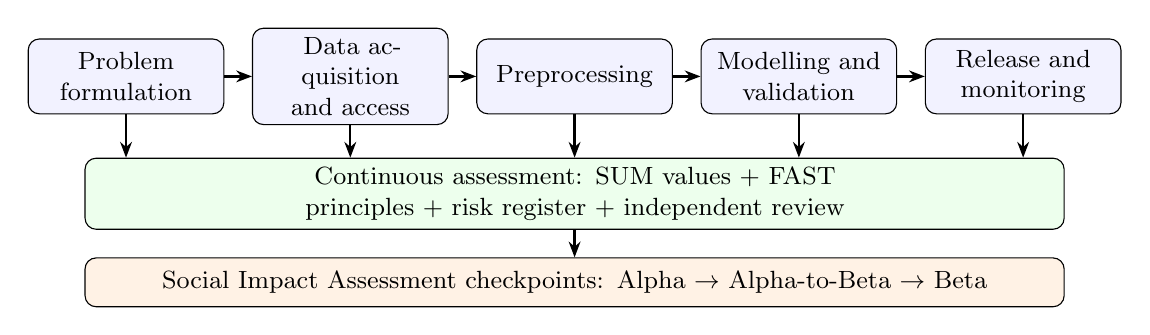
\begin{tikzpicture}[
    node distance=0.35cm,
    stage/.style={draw,rounded corners,align=center,text width=2.25cm,minimum height=0.95cm,font=\small,fill=blue!5},
    gate/.style={-{Stealth[length=2mm]},thick},
    band/.style={draw,rounded corners,align=center,fill=green!7,text width=12.2cm,minimum height=0.62cm,font=\small}
]
\node[stage] (p) {Problem\\ formulation};
\node[stage,right=of p] (d) {Data acquisition\\ and access};
\node[stage,right=of d] (x) {Preprocessing};
\node[stage,right=of x] (m) {Modelling and\\ validation};
\node[stage,right=of m] (r) {Release and\\ monitoring};
\draw[gate] (p) -- (d);
\draw[gate] (d) -- (x);
\draw[gate] (x) -- (m);
\draw[gate] (m) -- (r);
\node[band,below=0.55cm of x] (sf) {Continuous assessment: SUM values + FAST principles + risk register + independent review};
\node[band,below=0.35cm of sf,fill=orange!10] (sia) {Social Impact Assessment checkpoints: Alpha $\rightarrow$ Alpha-to-Beta $\rightarrow$ Beta};
\draw[gate] (p.south) -- (p.south |- sf.north);
\draw[gate] (d.south) -- (d.south |- sf.north);
\draw[gate] (x.south) -- (x.south |- sf.north);
\draw[gate] (m.south) -- (m.south |- sf.north);
\draw[gate] (r.south) -- (r.south |- sf.north);
\draw[gate] (sf) -- (sia);
\end{tikzpicture}
\caption{Proposed PBG structure for BrainWaveNet. Ethical review is continuous, with formal SIA checkpoints at key lifecycle transitions.}
\label{fig:pbg}
\end{figure}

Alpha decides whether to pursue the problem; Alpha-to-Beta governs controlled release; Beta reassesses real-world evidence. Insufficient evidence triggers pause, redesign or termination.

\subsection{Documented gaps and corrective priorities}
The following priorities address evidence gaps; they do not imply intentional misconduct or proven harm.

\begin{itemize}
\item \textbf{Autistic participation (SUM Respect/Connect):} establish accessible, paid co-design before defining any new intended use.
\item \textbf{Subgroup fairness (FAST Fairness):} report performance and uncertainty by age, sex, site and relevant clinical groups; compare included and excluded participants.
\item \textbf{Test-set governance (FAST Accountability):} inspect when repository test metrics are calculated and document a strictly independent final evaluation. The current concern is not proof of leakage.
\item \textbf{Reproducibility (FAST Transparency):} investigate paper--repository output differences and publish a tested, versioned reproduction package.
\item \textbf{Clinical safety (SUM Protect/Care):} prohibit diagnostic use until independent external validation, demonstrated patient-relevant benefit and clinical safety governance are in place.
\item \textbf{Resource impact (FAST Sustainability):} measure computational, MRI access and maintenance costs against the expected benefit.
\end{itemize}

\section{Conclusion}
BrainWaveNet is a research prototype, but its reported ABIDE-I results do not justify clinical diagnosis or autonomous decision-making. The assessment identifies several limitations: no documented autistic co-design, no reported subgroup or independent external clinical validation, incomplete reproducibility evidence, and no documented operational accountability or real-world monitoring. These are gaps in the available evidence and governance arrangements; they should not be treated as proof that harm has already occurred.

The appropriate next step is to restrict the project to research and apply the proposed PBG framework. The project should pass the problem, data, preprocessing, validation and release stages, with SUM and FAST reviews and SIA checkpoints at Alpha, Alpha-to-Beta and Beta. Clinical use should remain prohibited unless autistic stakeholders and clinicians support the proposed purpose and independent evidence demonstrates acceptable safety, fairness and benefit.

The immediate priorities are to establish meaningful autistic participation, define a clear research or clinical purpose, examine cohort selection and site effects, protect an independent test set, investigate differences between the paper and repository, and assign responsibility for safety and release decisions. Any future clinical pilot should be limited, supervised and reversible. Its outputs must be clearly described as research predictions rather than diagnoses. Monitoring should include subgroup performance, possible harms and a process through which affected people can raise concerns. If these conditions cannot be met, the responsible decision is not to deploy the model. BrainWaveNet may therefore have value as a research method, but the current evidence does not support its use as a clinical decision-support system.

\printbibliography[heading=bibintoc,title={References}]
\end{document}